\documentclass{article}

% if you need to pass options to natbib, use, e.g.:
% \PassOptionsToPackage{numbers, compress}{natbib}
% before loading nips_2017
%
% to avoid loading the natbib package, add option nonatbib:

\usepackage[nonatbib, final]{nips_2017}

% to compㅁle a camera-ready version, add the [final] option, e.g.:
\usepackage[utf8]{inputenc} % allow utf-8 input
\usepackage[T1]{fontenc}    % use 8-bit T1 fonts
\usepackage{hyperref}       % hyperlinks
\usepackage{url}            % simple URL typesetting
\usepackage{booktabs}       % professional-quality tables
\usepackage{amsfonts}       % blackboard math symbols
\usepackage{nicefrac}       % compact symbols for 1/2, etc.
\usepackage{microtype}      % microtypography
\usepackage{amsmath, amssymb, amsfonts, amsthm}
\usepackage{graphicx} % for pdf, bitmapped graphics files
\usepackage{subcaption}
\usepackage[font=small]{caption}

% Some reference styles
\newcommand{\eref}[1]{(\ref{#1})}% Equation
\newcommand{\aref}[1]{Algorithm~\ref{#1}}% Algorithm
\newcommand{\sref}[1]{Section~\ref{#1}}% Section
\newcommand{\figref}[1]{Figure~\ref{#1}}% Figure
\newcommand{\tabref}[1]{Table~\ref{#1}}% Table

\DeclareMathOperator*{\argmax}{arg\,max}
\DeclareMathOperator*{\argmin}{arg\,min}
\bibliographystyle{ieeetr}

\title{Milestone Report: Bayesian-Adaptive Deep Reinforcement Learning via Ensemble Learning}

% The \author macro works with any number of authors. There are two
% commands used to separate the names and addresses of multiple
% authors: \And and \AND.
%
% Using \And between authors leaves it to LaTeX to determine where to
% break the lines. Using \AND forces a line break at that point. So,
% if LaTeX puts 3 of 4 authors names on the first line, and the last
% on the second line, try using \AND instead of \And before the third
% author name.

\author{
  Gilwoo Lee \\ \texttt{gilwoo@cs.uw.edu} \\
  %% examples of more authors
  \And
  Jeongseok Lee \\ \texttt{jslee02@cs.uw.edu} \\
  \And
  Brian Hou \\ \texttt{bhou@cs.uw.edu} \\
  \And
  Aditya Vamsikrishna \\ \texttt{adityavk@cs.uw.edu} \\
}

\begin{document}
% \nipsfinalcopy is no longer used

\maketitle

\section{Introduction}
While reinforcement learning is capable of controlling complex autonomous systems, RL algorithms typically require huge amounts of data, can overfit to a particular task, or may learn brittle policies that are prone to disturbances. One of the main challenges that needs to be addressed is to train a policy that is robust to various model uncertainties and disturbances. In this project, we aim to address this challenge via an ensemble policy for Bayes-Adaptive Reinforcement Learning~\cite{ghavamzadeh2015bayesian}.

We assume that there exists a latent physics variable $\phi$ which determines the transition function of the underlying MDP, i.e., the transition function  $P(s',\phi' |s, \phi, a)$ is now a function of state, action, and $\phi$. We would like to learn a policy which maximizes the long term reward given $\phi$. Formally, this is called a Bayes-Adaptive MDP~\cite{ghavamzadeh2015bayesian, ross2008bayes, guez2012efficient}, defined by a tuple $\langle \mathcal{S}', \mathcal{A}, P, P_0, R \rangle$ where
\begin{itemize}
\item $\mathcal{S'} = \mathcal{S}\times \Phi$ is the set of hyper-states (states, physics variable),
\item $\mathcal{A}$ is the set of actions,
\item $P(s',\phi'|s, \phi, a)$ is the transition function between hyper-states, conditioned
on action $a$ being taken in hyper-state $(s, \phi)$,
\item $P_0\in \mathcal{P}(\mathcal{S} \times \Phi)$ combines the initial distribution over hyper-states,
\item $R(s, \phi, a)$ represents the reward obtained when action $a$ is
taken in hyper-state $(s,\phi)$.
\end{itemize}

We would like to find the optimal policy for the following Bellman equaton:
\begin{equation}\label{eq:rl}
V^*(s, \phi) = \max_a \mathbb{E} \bigg[R(s, a, \phi) + \gamma \sum_{s', \phi'}P(s',\phi'|s, \phi, a)V^*(s', \phi') \bigg].
\end{equation}

We make a simplification to the BARL formulation. We assume that the latent variable $\phi$ is either constant or the rate of change is slow enough that approximating the long-term value with a determinized $\phi$ is a reasonable short-term approximation for choosing one-step action, i.e. we can treat $V^*(s_t, \phi_t) \approx V^*(s_t, \phi_{t:\infty})$ for the purpose of one-step Bellman update.

This assumption allows us to simplify BARL with an ensemble policy learning method. At a high level, we have a network that updates the \emph{belief} of the physics parameters at time $t$,
\begin{align*}
b(\phi_t) = P(\phi_t|s_{t-1}, \phi_{t-1}, a_{t-1})
\end{align*}
which is then used to compute the best policy from an ensemble of $\phi$-dependent optimal policies, i.e., $\pi^*(\cdot;\phi)$ and $V^*(\cdot;\phi)$ are computed with typical RL algorithms for MDPs. Then the remaining task is to compute the one-step best action $a$:
\begin{align}\label{eq:barl}
 a^* &= \argmax_{a} \mathbb{E}_{\phi \sim b(\phi)} \bigg[R(s, a, \phi) + \gamma \sum_{s', \phi'}P(s',\phi'|s, \phi, a)V^{*'}(s', \phi') \bigg].
\end{align}

We model $b_\phi$ as a network capable of modeling evolving state change, e.g., Recurrent Neural Networks, or as a Bayes filter. At the low level, we plan to discretize $\Phi$ and have one actor-critic network per discretized value of $\phi$: each critic estimates $V^*(\cdot;\phi)$ and each actor has an optimal policy for a particular discretized value of $\pi^*(\cdot;\phi)$. Given $b_\phi$ and the set of value-function approximators, it is straightforward to compute (\ref{eq:barl}).

\section{Background}
Our work is closely related to QMDP~\cite{littman1995learning, karkus2017qmdp} which is an approximation for POMDP. QMDP approximates POMDP by assuming fully-observable MDP after 1-step, and approximating the Q-value at the current belief state $b(s)$ as $Q_a(b) =\sum_s b(s)Q_{\text{MDP}}(s, a)$. In our problem setup, we have a belief over the physics parameters $\phi$ of the MDP, $b(\phi)$, and we compute the policy $Q_a(s;b) = \sum_\phi b(\phi)Q_{\text{MDP}}(s,a;\phi)$.

The BAMDP formulation is also similar to POMDP formulation used in POMDP-lite~\cite{chen2016pomdp} which assumes that the hidden state variables are constant or only change deterministically. In our case, the hidden state variables correspond to the physics parameters $\phi$. The authors of POMDP-lite have shown that such formulation is ``equivalent to a set of fully observable Markov decision processes indexed by a hidden parameter''~\cite{chen2016pomdp}, which, in our case, is a discretization of $\phi$.

\section{Milestones}
We have proposed the following milestones in our proposal:
\begin{itemize}
\item April 30 -- Set up all simulation environments in DART~\cite{lee2018dart} (including a kinematic simulation for the RACECAR)
\item May 15   -- Test algorithm on simulated OpenAI problems
\item May 22   -- Test algorithm on RACECAR in simulation
\item May 31   -- Run experiments on the real RACECAR
\end{itemize}

\section{RACECAR}
We are working on both simulation~(\figref{subfig:simcar}) and real-robot~(\figref{subfig:racecar}) platform for the RACECAR.
\begin{figure*}
 \begin{subfigure}[b]{0.49\textwidth}
   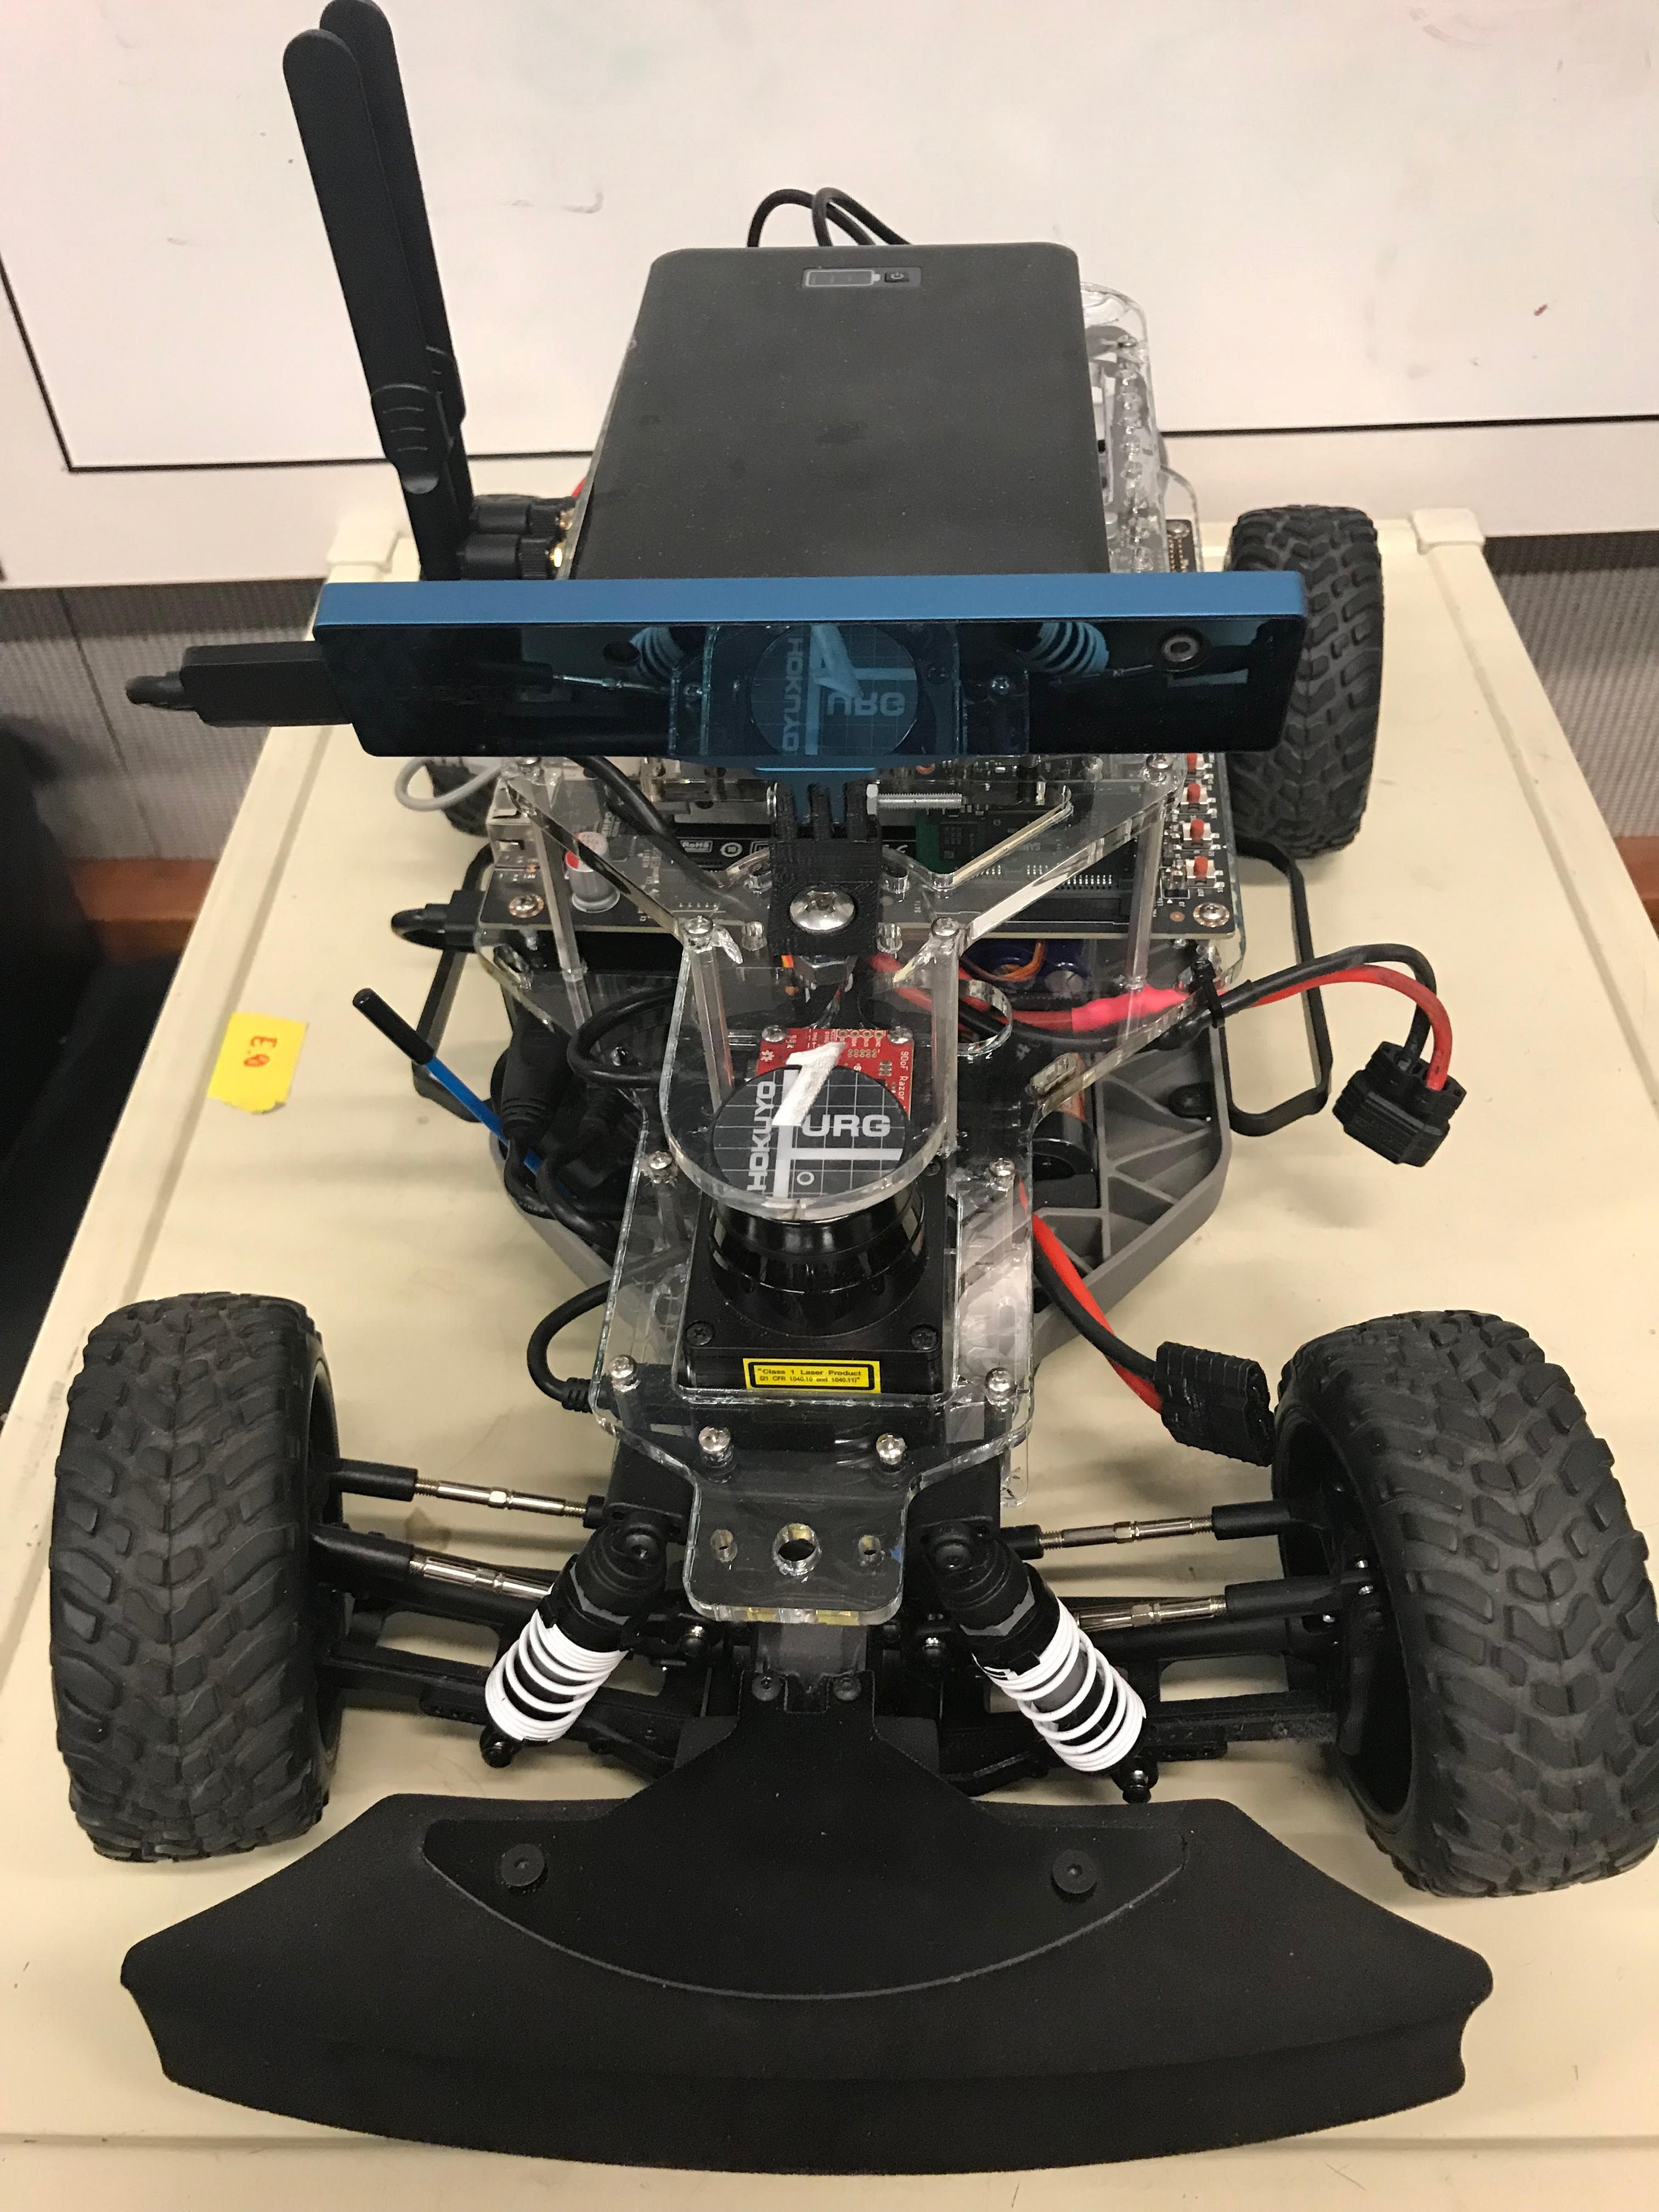
\includegraphics[width=1\linewidth]{figs/racecar.jpg}
   \caption{Simulated RACECAR in DART}
   \label{subfig:simcar}
 \end{subfigure}
 \hfill
 \begin{subfigure}[b]{0.49\textwidth}
   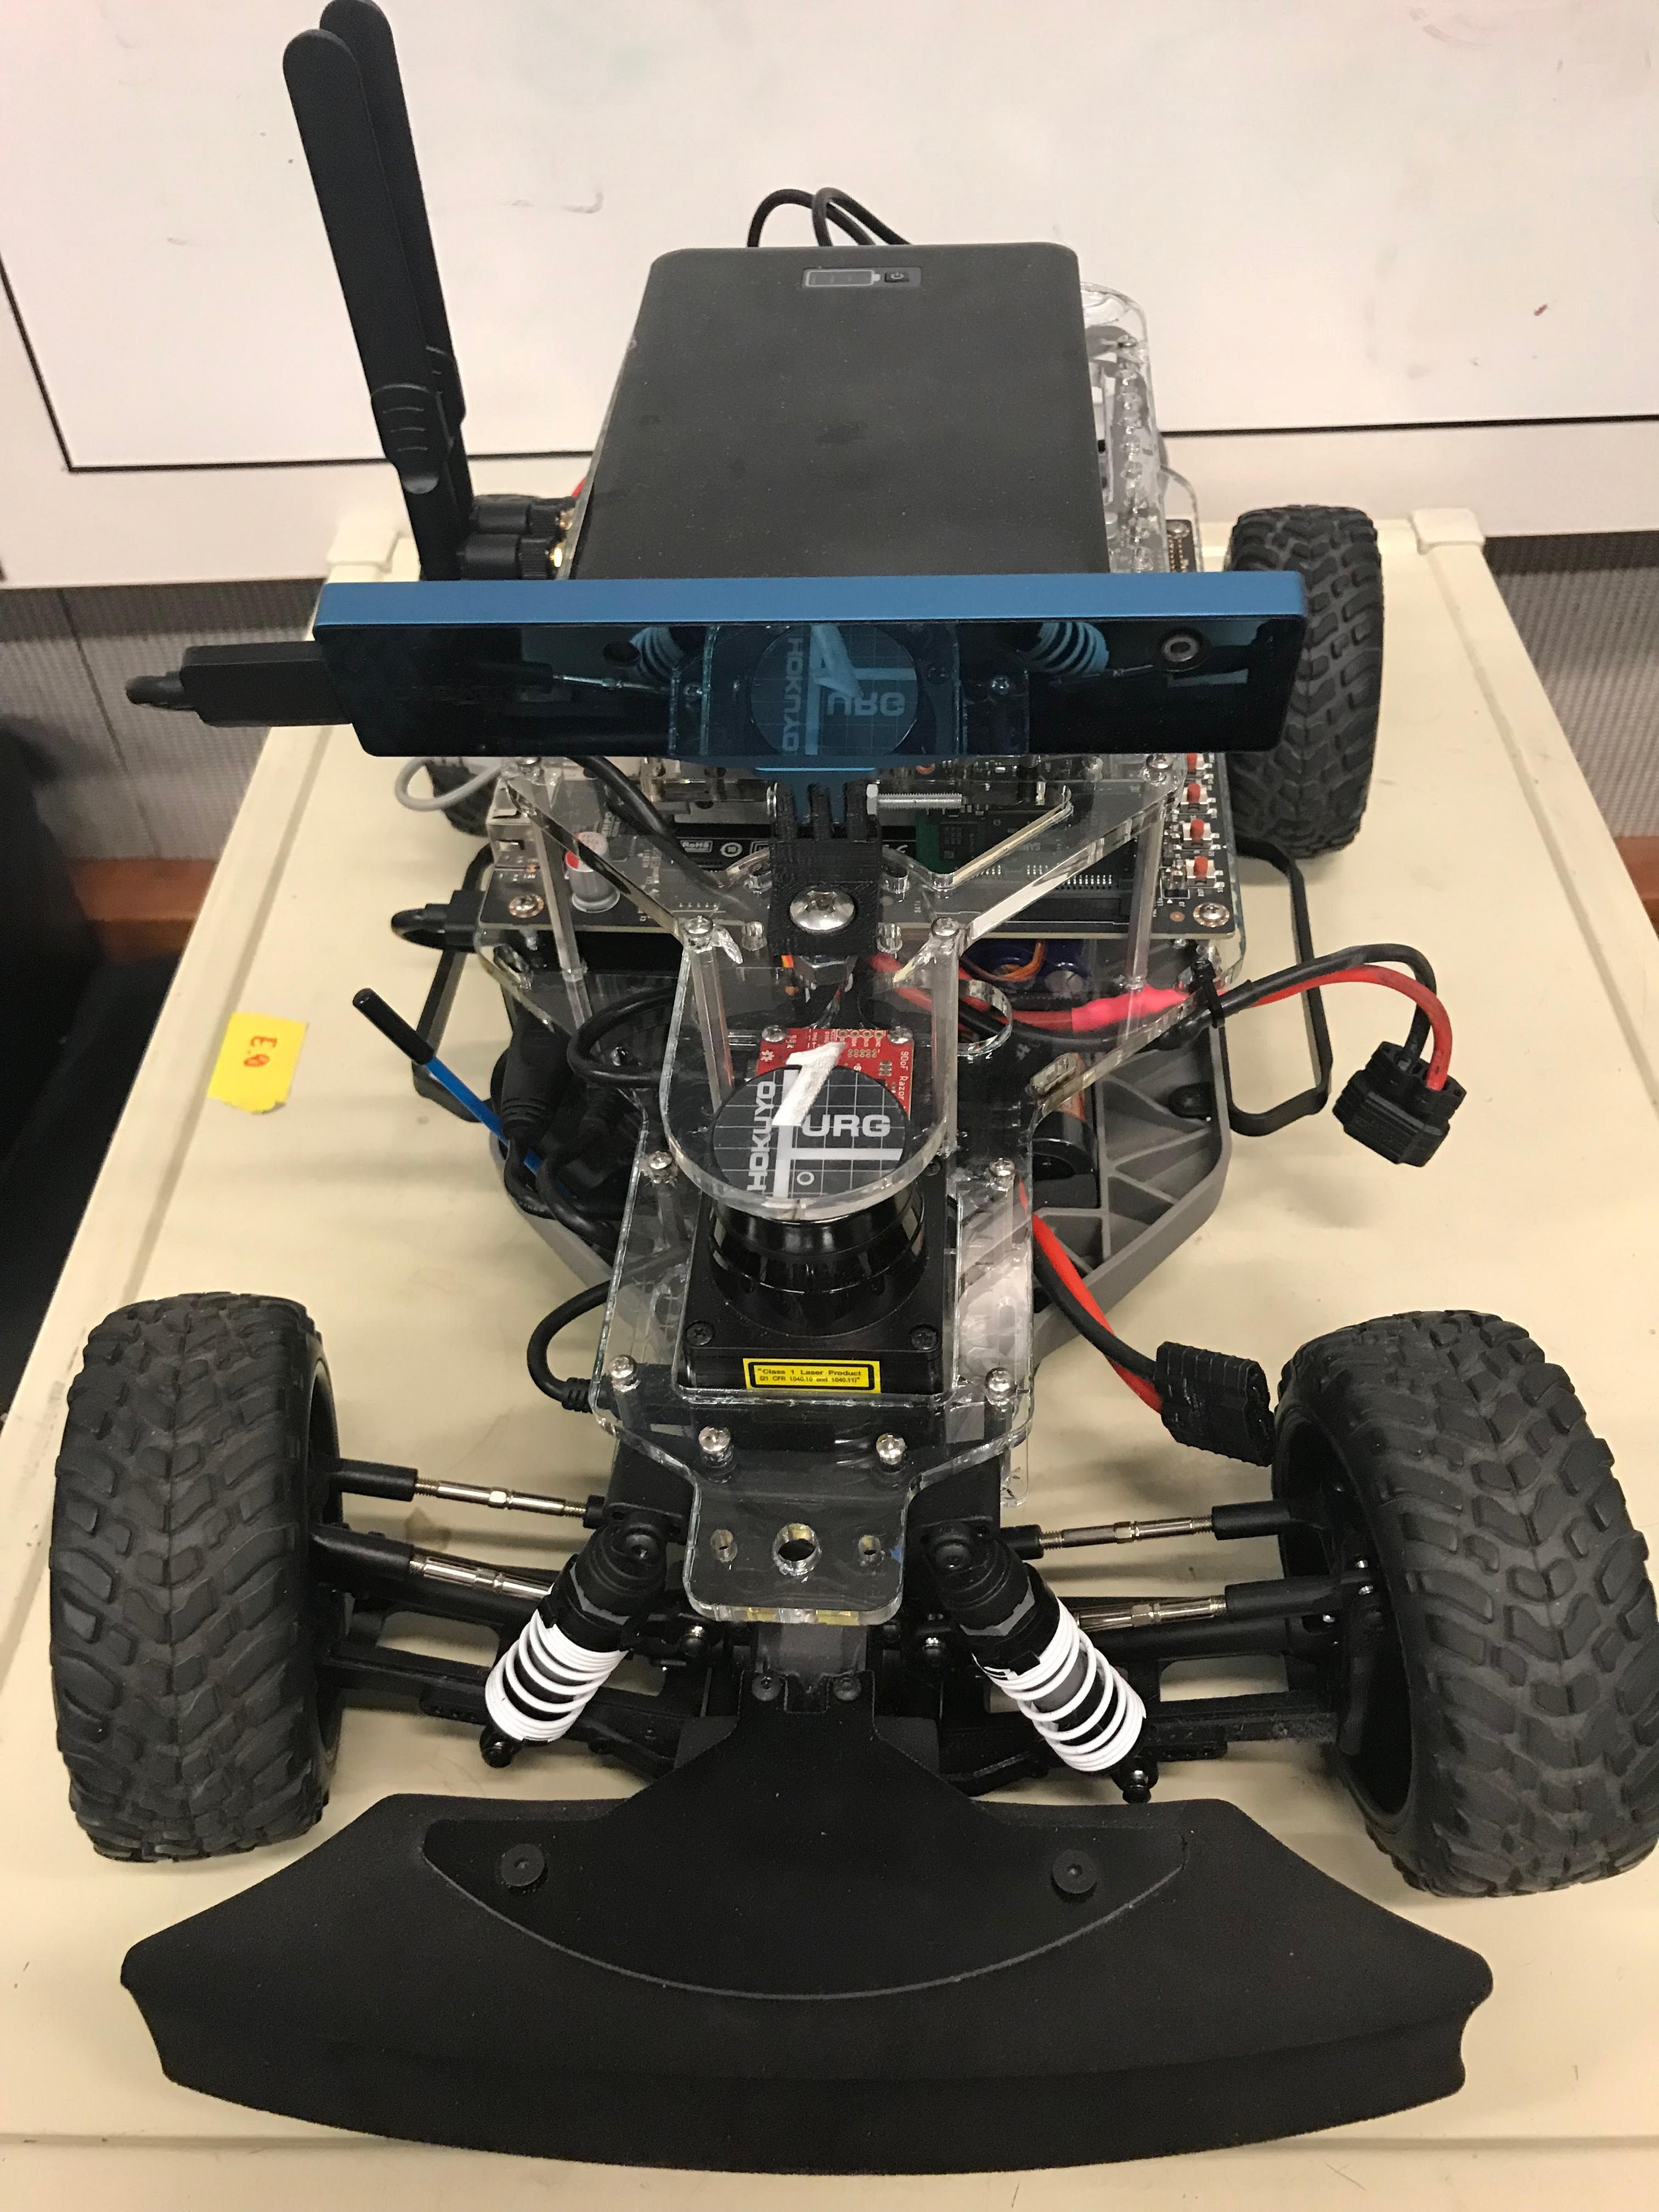
\includegraphics[width=1\linewidth]{figs/racecar.jpg}
   \caption{RACECAR}
   \label{subfig:racecar}
 \end{subfigure}
 \label{fig:racecar}
\caption{RACECAR}
\end{figure*}

The RACECAR is controlled by torque of the front wheels and position and velocity control of the steering angle. The goal of the task is to track a trajectory as fast as it can. The physics parameters we plan to change are mass of the car and friction coefficient between the car and the road, both of which affect the car dynamics significantly.

\section{Experiments}

We have setup a set of simulated examples and a set of RL algorithms to be utilized in our ensemble approach. For simualted examples, we have the following agents: \textbf{ant, reacher, swimmer, half-cheetah}, each with a predefined reward function defined similar to those given by OpenAI Gym~\cite{openai}. We are utilizing TRPO~\cite{trpo}, VPG, DDPG~\cite{ddpg} provide by \texttt{rllab}~\cite{duan2016benchmarking} as a set of algorithms to be utilized in our ensemble approach. In addition, we plan to implement PPO and a PID controller for RACECAR.

Our algorithm will be compared against two classes of algorithms: (1) sample-based algorithms which chooses an MDP and commits to this policy for a fixed horizon, and (2) ensemble algorithms which trains a policy over an ensemble of MDP models. A greedy algorithm which chooses the maximum-likely MDP, or one that samples from a posterior distribution of MDPs given previous observations (e.g. Posterior Sampling Reinforcement Learning \cite{psrl}) would fall into the former, and EPOpt\cite{rajeswaran2016epopt} and Ensemble-CIO~\cite{ensemble-cio} would fall into the latter.

\bibliography{intuitive_physics}

\end{document}
